\section{Даталогическая модель}\label{sec:datalogical-model}


\renewcommand{\tab}{\hspace{1cm}}

\setlist[enumerate, 1]{align=left, leftmargin=0cm, labelindent=1cm, listparindent=1cm, labelwidth=*, itemindent=2cm}
\setlist[itemize, 1]{align=left, leftmargin=1cm, labelindent=2cm, listparindent=1cm, labelwidth=*, itemindent=2cm}


\subsection{Обзор СУБД <<PostgreSQL>>}

PostgreSQL \cite{postgrespro} -- это свободно распространяемая объектно-реляционная система управления базами данных, наиболее развитая в мире из СУБД с открытым исходным кодом и являющаяся реальной альтернативой коммерческим базам данных.

Благодаря свободной лицензии, PostgreSQL разрешается бесплатно использовать, изменять и распространять всем и для любых целей -- личных, коммерческих или учебных.

PostgreSQL обладает рядом особенностей:
\begin{enumerate}
    \item \textbf{Функции}
    
    \tab Функции являются блоками кода, исполняемыми на сервере, а не на клиенте БД. Хотя они могут писаться на чистом SQL, реализация дополнительной логики, например, условных переходов и циклов, выходит за рамки собственно SQL и требует использования некоторых языковых расширений. Функции могут писаться с использованием одного из следующих языков:
    \begin{itemize}
        \item Встроенный процедурный язык PL/pgSQL, во многом аналогичный языку PL/SQL, используемому в СУБД Oracle.
        \item Скриптовые языки -- PL/Lua, PL/LOLCODE, PL/Perl, PL/PHP, PL/Python, PL/Ruby, PL/sh, PL/Tcl и PL/Scheme.
        \item Классические языки -- C, C++, Java (через модуль PL/Java).
        \item Статистический язык R (через модуль PL/R).
    \end{itemize}

    \tab PostgreSQL допускает использование функций, возвращающих набор записей, который далее можно использовать так же, как и результат выполнения обычного запроса.
    
    \tab Функции могут выполняться как с правами их создателя, так и с правами текущего пользователя.
    
    \tab Иногда функции отождествляются с хранимыми процедурами, однако между этими понятиями есть различие. С девятой версии возможно написание автономных блоков, которые позволяют выполнять код на процедурных языках без написания функций, непосредственно в клиенте.


    \item \textbf{Триггеры}
    
    \tab Триггеры определяются как функции, инициируемые DML-операциями. Например, операция \texttt{INSERT} может запускать триггер, проверяющий добавленную запись на соответствия определённым условиям. При написании функций для триггеров могут использоваться различные языки программирования (см. выше). % нужна ссылка
    
    \tab Триггеры ассоциируются с таблицами. Множественные триггеры выполняются в алфавитном порядке.


    \item \textbf{Механизм правил}

    \tab Механизм правил (англ. \textit{rules}) представляет собой механизм создания пользовательских обработчиков не только DML-операций, но и операции выборки. Основное отличие от механизма триггеров заключается в том, что правила срабатывают на этапе разбора запроса, до выбора оптимального плана выполнения и самого процесса выполнения. Правила позволяют переопределять поведение системы при выполнении SQL-операции к таблице. Хорошим примером является реализация механизма представлений (англ. \textit{views}): при создании представления создается правило, которое определяет, что вместо выполнения операции выборки к представлению система должна выполнять операцию выборки к базовой таблице / таблицам с учетом условий выборки, лежащих в основе определения представления. Для создания представлений, поддерживающих операции обновления, правила для операций вставки, изменения и удаления строк должны быть определены пользователем.


    \item \textbf{Индексы}

    \tab В PostgreSQL имеется поддержка индексов следующих типов: B-дерево, хэш, R-дерево, GiST, GIN. При необходимости можно создавать новые типы индексов, хотя это далеко не тривиальный процесс. Индексы в PostgreSQL обладают следующими свойствами:
    \begin{itemize}
        \item возможен просмотр индекса не только в прямом, но и в обратном порядке – создание отдельного индекса для работы конструкции \texttt{ORDER BY ... DESC} не нужно;
        \item возможно создание индекса над несколькими столбцами таблицы, в том числе над столбцами различных типов данных;
        \item индексы могут быть функциональными, то есть строиться не на базе набора значений некоего столбца / столбцов, а на базе набора значений функции от набора значений;
        \item индексы могут быть частичными, то есть строиться только по части таблицы (по некоторой её проекции); в некоторых случаях это помогает создавать намного более компактные индексы или достигать улучшения производительности за счёт использования разных типов индексов для разных (например, с точки зрения частоты обновления) частей таблицы;
        \item планировщик запросов может использовать несколько индексов одновременно для выполнения сложных запросов.
    \end{itemize}


    \item \textbf{Многоверсионность (MVCC)}

    \tab PostgreSQL поддерживает одновременную модификацию БД несколькими пользователями с помощью механизма MultiVersion Concurrency Control (MVCC). Благодаря этому соблюдаются требования ACID, и практически отпадает нужда в блокировках чтения.


    \item \textbf{Расширение}

    \tab Расширение PostgreSQL для собственных нужд возможно практически в любом аспекте. Есть возможность добавлять собственные преобразования типов, типы данных, домены (пользовательские типы с изначально наложенными ограничениями), функции (включая агрегатные), индексы, операторы (включая переопределение уже существующих) и процедурные языки.


    \item \textbf{Наследование}

    \tab Наследование в PostgreSQL реализовано на уровне таблиц. Таблицы могут наследовать характеристики и наборы полей от других таблиц (родительских). При этом данные, добавленные в порождённую таблицу, автоматически будут участвовать (если это не указано отдельно) в запросах к родительской таблице.


    \item \textbf{Пользовательские объекты}

    \tab PostgreSQL может быть расширен пользователем для собственных нужд практически в любом аспекте. Есть возможность добавлять собственные \cite{web-creator}:
    \begin{itemize}
        \item преобразования типов;
        \item типы данных;
        \item домены (пользовательские типы с изначально наложенными ограничениями);
        \item функции (включая агрегатные);
        \item индексы;
        \item операторы (включая переопределение уже существующих);
        \item процедурные языки.
    \end{itemize}
\end{enumerate}


\subsection{Описание таблиц базы данных}


\newcolumntype{R}{>{\centering\arraybackslash}p{0.4 \textwidth}}


\begin{enumerate}
    \item Таблица \textbf{<<Телефонные номера>>} (phone\_numbers)
    
    \renewcommand{\arraystretch}{1.5}
    \begin{xltabular}[h]{\textwidth}{|C|C|C|}
        \caption{Таблица <<Телефонные номера>>} \\
        \hline
        \textbf{Название атрибута}   & \textbf{Тип}         & \textbf{Свойство} \\
        \hline \endhead
        \texttt{phone\_number}       & \texttt{bigint}      & \texttt{NOT NULL} \\ \hline
        \texttt{subscriber\_account} & \texttt{varchar(20)} & \texttt{NULL}     \\ \hline
    \end{xltabular}

    \renewcommand{\arraystretch}{1.5}
    \begin{xltabular}[h]{\textwidth}{|X|X|}
        \caption{Дополнительные свойства атрибутов таблицы <<Телефонные номера>>} \\
        \hline
        \textbf{Первичный ключ}                                  & \texttt{phone\_number}                               \\ \hline
        \textbf{Внешние ключи}                                   & \texttt{subscriber\_account}                         \\ \hline
        \textbf{Валидация атрибута \texttt{phone\_number}}       & \texttt{\textasciicircum{}\textbackslash{}d\{10\}\$} \\ \hline
        \textbf{Маска атрибута \texttt{phone\_number}}           & \texttt{+7 (999) 999-99-99}                          \\ \hline
        \textbf{Валидация атрибута \texttt{subscriber\_account}} & \texttt{\textasciicircum{}\textbackslash{}d\{20\}\$} \\ \hline
        \textbf{Маска атрибута \texttt{subscriber\_account}}     & \texttt{99999999999999999999}                        \\ \hline
    \end{xltabular}


    \item Таблица \textbf{<<Тарифы>>} (tariffs)
    
    \renewcommand{\arraystretch}{1.5}
    \begin{xltabular}[h]{\textwidth}{|C|C|C|}
        \caption{Таблица <<Тарифы>>} \\
        \hline
        \textbf{Название атрибута}  & \textbf{Тип}          & \textbf{Свойство} \\
        \hline \endhead
        \texttt{name}               & \texttt{varchar(64)}  & \texttt{NOT NULL} \\ \hline
        \texttt{subscription\_fee}  & \texttt{smallint}     & \texttt{NOT NULL} \\ \hline
        \texttt{internet\_traffic}  & \texttt{decimal(4,2)} & \texttt{NOT NULL} \\ \hline
        \texttt{minutes}            & \texttt{smallint}     & \texttt{NOT NULL} \\ \hline
        \texttt{sms}                & \texttt{smallint}     & \texttt{NOT NULL} \\ \hline
    \end{xltabular}

    \renewcommand{\arraystretch}{1.5}
    \begin{xltabular}[h]{\textwidth}{|X|X|}
        \caption{Дополнительные свойства атрибутов таблицы <<Тарифы>>} \\
        \hline
        \textbf{Первичный ключ}                                  & \texttt{name}                               \\ \hline
        \textbf{Валидация атрибута \texttt{name}}                & \texttt{\textasciicircum{}{[} \textbackslash{}wА-ЯЁа-яё!?,\%-{]}\{2,64\}\$} \\ \hline
        \textbf{Валидация атрибута \texttt{subscription\_fee}}   & \texttt{+7 (999) 999-99-99}                          \\ \hline
        \textbf{Валидация атрибута \texttt{subscriber\_account}} & \texttt{\textasciicircum{}\textbackslash{}d\{20\}\$} \\ \hline
        \textbf{Маска атрибута \texttt{subscriber\_account}}     & \texttt{99999999999999999999}                        \\ \hline
    \end{xltabular}

   

    \item Таблица \textbf{<<Клиенты>>} (clients)
    
    \renewcommand{\arraystretch}{1.5}
    \begin{xltabular}[h]{\textwidth}{|R|C|C|}
        \caption{Таблица <<Клиенты>>} \\
        \hline
        \textbf{Название атрибута}           & \textbf{Тип}          & \textbf{Свойство} \\
        \hline \endhead
        \texttt{passport}                    & \texttt{bigint}       & \texttt{NOT NULL} \\
        \hline
        \texttt{full\_name}                  & \texttt{varchar(128)} & \texttt{NOT NULL} \\
        \hline
        \texttt{place\_of\_registration\_id} & \texttt{serial}       & \texttt{NOT NULL} \\
        \hline
        \texttt{date\_of\_birth}             & \texttt{date}         & \texttt{NOT NULL} \\
        \hline
    \end{xltabular}

    \tab Первичный ключ: \texttt{passport}.

    \tab Внешние ключи: \texttt{place\_of\_registration\_id}.
    

    \item \textbf{Таблица <<Места прописок>>} (places\_of\_registration)
    
    \renewcommand{\arraystretch}{1.5}
    \begin{xltabular}[h]{\textwidth}{|R|C|C|}
        \caption{Таблица <<Места прописок>>} \\
        \hline
        \textbf{Название атрибута}       & \textbf{Тип}          & \textbf{Свойство} \\
        \hline \endhead
        \texttt{id}                      & \texttt{serial}       & \texttt{NOT NULL} \\
        \hline
        \texttt{place\_of\_registration} & \texttt{varchar(255)} & \texttt{NOT NULL} \\
        \hline
    \end{xltabular}

    \tab Первичный ключ: \texttt{id}.

    \tab Внешние ключи: \texttt{place\_of\_registration\_id}.
    

    \item Таблица \textbf{<<Абоненты>>} (subscribers)
    
    \renewcommand{\arraystretch}{1.5}
    \begin{xltabular}[h]{\textwidth}{|C|C|C|}
        \caption{Таблица <<Абоненты>>} \\
        \hline
        \textbf{Название атрибута} & \textbf{Тип}           & \textbf{Свойство}  \\
        \hline \endhead
        \texttt{account}           & \texttt{varchar(20)}   & \texttt{NOT NULL}  \\
        \hline
        \texttt{balance}           & \texttt{decimal(8, 2)} & \texttt{DEFAULT 0} \\
        \hline
        \texttt{connected\_tariff} & \texttt{varchar(64)}   & \texttt{NULL}      \\
        \hline
        \texttt{passport}          & \texttt{bigint}        & \texttt{NOT NULL}  \\
        \hline
    \end{xltabular}

    \tab Первичный ключ: \texttt{account}.

    \tab Внешние ключи: \texttt{passport}, \texttt{connected\_tariff}.


    \item Таблица \textbf{<<Пользователи>>} (users)
    
    \renewcommand{\arraystretch}{1.5}
    \begin{xltabular}[h]{\textwidth}{|C|C|C|}
        \caption{Таблица <<Пользователи>>} \\
        \hline
        \textbf{Название атрибута} & \textbf{Тип}         & \textbf{Свойство} \\
        \hline \endhead
        \texttt{login}             & \texttt{varchar(32)} & \texttt{NOT NULL} \\
        \hline
        \texttt{password}          & \texttt{varchar(32)} & \texttt{NOT NULL} \\
        \hline
        \texttt{user\_type\_id}    & \texttt{serial}      & \texttt{NOT NULL} \\
        \hline
    \end{xltabular}

    \tab Первичный ключ: \texttt{login}.

    \tab Внешние ключи: \texttt{user\_type\_id}.


    \item Таблица \textbf{<<Типы пользователей>>} (user\_types)
    
    \renewcommand{\arraystretch}{1.5}
    \begin{xltabular}[h]{\textwidth}{|C|C|C|}
        \caption{Таблица <<Типы пользователей>>} \\
        \hline
        \textbf{Название атрибута} & \textbf{Тип}         & \textbf{Свойство} \\
        \hline \endhead
        \texttt{id}                & \texttt{serial}      & \texttt{NOT NULL} \\
        \hline
        \texttt{user\_type}        & \texttt{varchar(32)} & \texttt{NOT NULL} \\
        \hline
    \end{xltabular}

    \tab Первичный ключ: \texttt{id}.
\end{enumerate}


\subsection{Схема данных}


\begin{figure}[H]
    \center{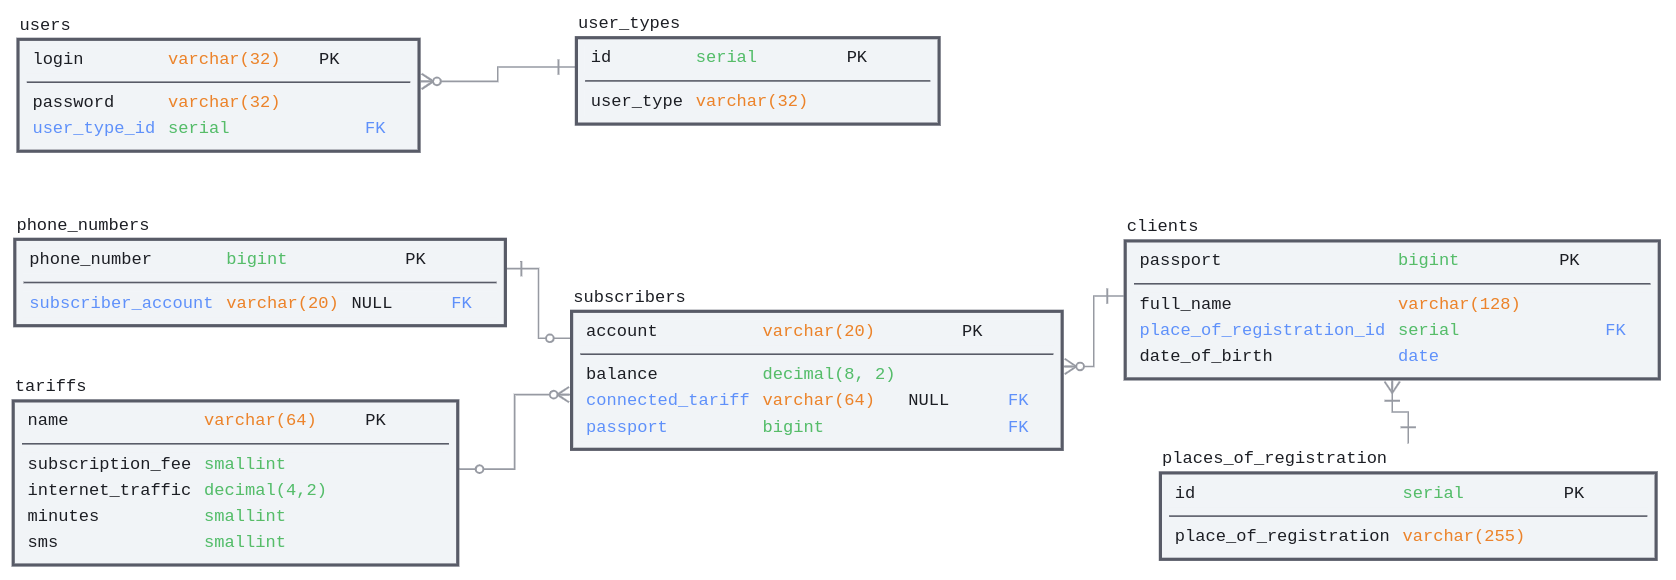
\includegraphics[scale=0.28]{screenshots/scheme}}
    \caption{Схема данных}
    \label{fig:schema}
\end{figure}


